\chapter{Metodologia}
\label{cap:metodologia}

\section{Escopo do Experimento}
\label{sec:escopo}

O escopo deste experimento é definido a partir do paradigma \textit{Goal Question Metric} (GQM) \cite{basili1994gqm}. O objetivo é formulado como: analisar \textit{guardrails} baseados em LLM, com o propósito de avaliá-los, com relação à eficácia na classificação de conteúdo prejudicial, do ponto de vista de pesquisadores e desenvolvedores, no contexto de modelos submetidos a diferentes níveis de quantização via GPTQ e AWQ, operando sobre entradas em inglês e em português brasileiro.

\section{Design Experimental}
\label{sec:design}

Este trabalho adota o framework de experimentos controlados em Engenharia de Software proposto por \citeonline{wohlin2012experimentation}, adaptado para o contexto de experimentos computacionais com modelos de linguagem. Nessa adaptação, os modelos de linguagem assumem o papel de sujeitos empíricos, pois são eles que executam a tarefa de classificação sobre os objetos do experimento. Essa escolha é declarada explicitamente pois o framework original foi concebido para experimentos com participantes humanos \cite{wohlin2012experimentation}, e sua adaptação para agentes computacionais implica diferenças metodológicas discutidas ao longo desta seção.

O experimento segue um design fatorial completo \cite{wohlin2012experimentation}, em que todas as combinações possíveis entre os fatores são avaliadas, totalizando 40 configurações experimentais, conforme ilustrado na Figura~\ref{fig:design-fatorial}. A ordem de inferência não foi aleatorizada, pois, sob as restrições do protocolo definido na Seção~\ref{sec:protocolo}, cada prompt é processado de forma independente, eliminando efeitos de aprendizado ou fadiga \cite{wohlin2012experimentation} que justificariam a aleatorização em experimentos com sujeitos humanos.

\begin{figure}[h!]
	\Caption{\label{fig:design-fatorial} Design fatorial do experimento}
	\UFCfig{}{
		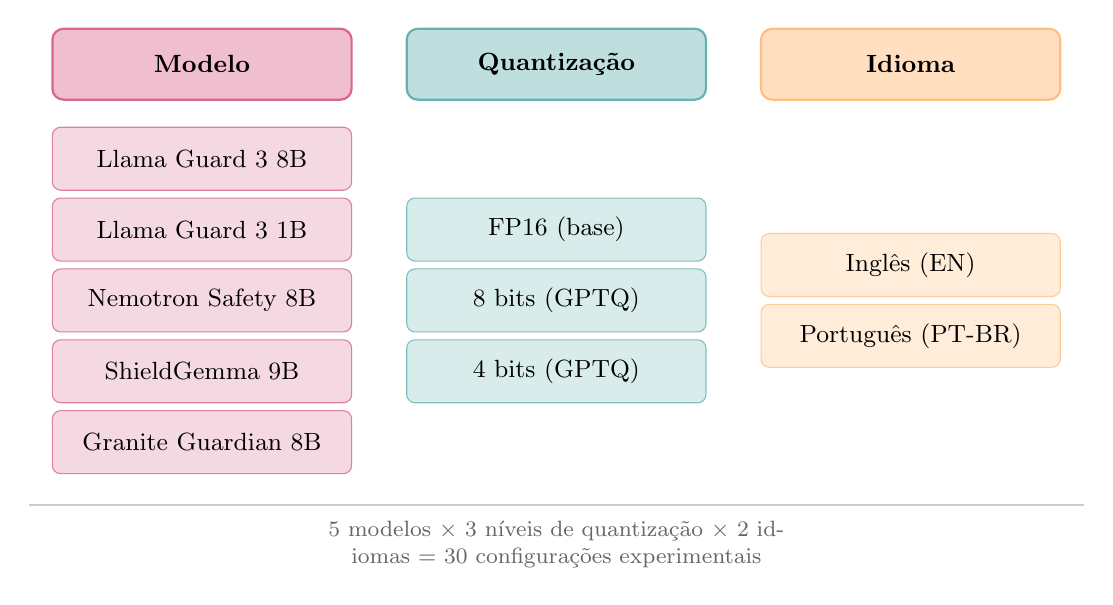
\begin{tikzpicture}[
			font=\small,
			factor/.style={rectangle, rounded corners=4pt, minimum width=3.8cm, minimum height=0.9cm, text centered, draw=black!60, thick},
			level/.style={rectangle, rounded corners=3pt, minimum width=3.8cm, minimum height=0.8cm, text centered, draw=black!40},
			modelo/.style={level, fill=purple!15, draw=purple!50},
			quant/.style={level, fill=teal!15, draw=teal!50},
			idioma/.style={level, fill=orange!15, draw=orange!40},
			fator_modelo/.style={factor, fill=purple!25, draw=purple!60},
			fator_quant/.style={factor, fill=teal!25, draw=teal!60},
			fator_idioma/.style={factor, fill=orange!25, draw=orange!50},
			]
			\node[fator_modelo] (fm) at (0,0)     {\textbf{Modelo}};
			\node[fator_quant]  (fq) at (4.5,0)   {\textbf{Quantização}};
			\node[fator_idioma] (fi) at (9,0)      {\textbf{Idioma}};
			\node[modelo] (m1) at (0,-1.2)  {Llama Guard 3 8B};
			\node[modelo] (m2) at (0,-2.1)  {Llama Guard 3 1B};
			\node[modelo] (m3) at (0,-3.0)  {Nemotron Safety 8B};
			\node[modelo] (m4) at (0,-3.9)  {ShieldGemma 9B};
			\node[modelo] (m5) at (0,-4.8)  {Granite Guardian 8B};
			\node[quant] (q1) at (4.5,-2.1) {FP16 (base)};
			\node[quant] (q2) at (4.5,-3.0) {8 bits (GPTQ)};
			\node[quant] (q3) at (4.5,-3.9) {4 bits (GPTQ)};
			\node[idioma] (i1) at (9,-2.55) {Inglês (EN)};
			\node[idioma] (i2) at (9,-3.45) {Português (PT-BR)};
			\draw[black!20, thick] (-2.2,-5.6) -- (11.2,-5.6);
			\node[text width=10cm, text centered, font=\footnotesize, text=black!60] 
			at (4.5,-6.1) 
			{5 modelos $\times$ 3 níveis de quantização $\times$ 2 idiomas = 30 configurações experimentais};
		\end{tikzpicture}
	}{
		\Fonte{Elaborado pelo autor.}
	}
\end{figure}

\subsection{Fatores e Tratamentos}
\label{sec:fatores}

Os fatores deste experimento são as variáveis independentes efetivamente manipuladas. Vale observar que o fator modelo assume um duplo papel neste design: os modelos são simultaneamente sujeitos, pois executam a tarefa de classificação, e um fator experimental, pois seu tipo é uma variável independente do experimento. Essa sobreposição é característica de estudos comparativos entre sistemas computacionais e não compromete o design fatorial adotado.

O primeiro fator é o \textbf{modelo}, cujos cinco níveis correspondem aos cinco \textit{guardrails} selecionados e detalhados na Seção~\ref{sec:modelos}. O segundo fator é o \textbf{nível de quantização}, com três níveis: precisão base em 16 bits (FP16), quantização em 8 bits e quantização em 4 bits, todos aplicados via GPTQ. O terceiro fator é o \textbf{idioma}, com dois níveis: inglês (EN) e português brasileiro (PT-BR).

Algumas variáveis independentes foram mantidas fixas ao longo de todo o experimento, 
não constituindo fatores, mas sendo registradas como variáveis de controle para 
garantir a reprodutibilidade dos resultados. São elas: temperatura de inferência 
fixada em zero, garantindo comportamento determinístico dos modelos; conjunto de 
calibração AWQ padronizado (Pile); e modo de classificação de entrada 
(\textit{input classification}), aplicado uniformemente a todos os modelos.


\subsection{Variáveis Dependentes}
\label{sec:variaveis}

As variáveis dependentes são as métricas que capturam o efeito dos tratamentos sobre o desempenho dos modelos na tarefa de classificação de conteúdo prejudicial. As métricas primárias são precisão (\textit{precision}), revocação (\textit{recall}) e F1-\textit{score}, calculadas para cada uma das 30 configurações experimentais resultantes do cruzamento entre cinco modelos, três níveis de quantização e dois idiomas. A métrica derivada central é o $\Delta$F1, definido como a diferença entre o F1 macro obtido em inglês e o F1 macro obtido em português brasileiro para uma mesma configuração de modelo e nível de quantização, operacionalizando diretamente a pergunta de pesquisa deste trabalho. As fórmulas e procedimentos de cálculo dessas métricas são detalhados na Seção~\ref{sec:metricas}.

\subsection{Objetos}
\label{sec:objetos}
Os objetos do experimento são os prompts de \textit{red-teaming} que compõem o conjunto de dados utilizado na avaliação. Cada prompt representa uma entrada submetida aos \textit{guardrails} para classificação binária entre seguro (\textit{safe}) e inseguro (\textit{unsafe}), e está disponível em duas versões linguísticas pareadas: inglês (EN) e português brasileiro (PT-BR). O mesmo conteúdo em ambos os idiomas permite isolar o efeito do idioma sobre o desempenho dos modelos, mantendo constante a intenção do prompt. O conjunto abrange tanto entradas benignas quanto entradas nocivas, cobrindo as 14 categorias de dano definidas na Seção~\ref{sec:dataset}, o que permite avaliar se os modelos discriminam corretamente o conteúdo em ambos os idiomas e níveis de quantização. Os detalhes sobre a composição, processo de deduplicação, reclassificação e tradução do conjunto de dados são apresentados na Seção~\ref{sec:dataset}.

\subsection{Sujeitos}
\label{sec:sujeitos}
Os sujeitos do experimento são os cinco \textit{guardrails} baseados em LLM selecionados para avaliação. No contexto deste trabalho, os modelos assumem o papel de sujeitos pois são eles que executam a tarefa de classificação sobre os objetos, emitindo julgamentos binários de segurança sob as restrições definidas no protocolo de inferência da Seção~\ref{sec:protocolo}. Os critérios de seleção, características e configurações de cada modelo são detalhados na Seção~\ref{sec:modelos}.

\section{Hipóteses}
\label{sec:hipoteses}

Este trabalho investiga quatro hipóteses sobre o comportamento de \textit{guardrails} baseados em LLM sob efeito de quantização em português brasileiro. Para cada hipótese, define-se formalmente a hipótese nula ($H_0$) e a hipótese alternativa ($H_1$), bem como o critério de avaliação adotado.

A primeira hipótese investiga se a quantização amplifica o \textit{gap} de desempenho entre inglês e português brasileiro:

\begin{itemize}
	\item[$H_0^1$:] A quantização não aumenta o \textit{gap} de desempenho entre idiomas, isto é, $\Delta$F1$_{\text{FP16}} \geq$ $\Delta$F1$_{\text{8bit}} \geq$ $\Delta$F1$_{\text{4bit}}$.
	\item[$H_1^1$:] A quantização amplifica o \textit{gap} de desempenho entre idiomas, isto é, $\Delta$F1 aumenta conforme o número de bits diminui.
\end{itemize}

A segunda hipótese investiga se modelos com \textit{safety fine-tuning} predominantemente em inglês apresentam maior \textit{gap} multilíngue no \textit{baseline} FP16:

\begin{itemize}
	\item[$H_0^2$:] O $\Delta$F1$_{\text{FP16}}$ não difere sistematicamente entre modelos multilíngues nativos e modelos com \textit{safety fine-tuning} predominantemente em inglês.
	\item[$H_1^2$:] Modelos com \textit{safety fine-tuning} predominantemente em inglês apresentam $\Delta$F1$_{\text{FP16}}$ maior do que modelos multilíngues nativos.
\end{itemize}

A terceira hipótese investiga se modelos de menor escala são mais suscetíveis à degradação multilíngue sob quantização:

\begin{itemize}
	\item[$H_0^3$:] O $\Delta$F1 do Llama Guard 3 1B não é superior ao $\Delta$F1 do Llama Guard 3 8B sob quantização.
	\item[$H_1^3$:] O $\Delta$F1 do Llama Guard 3 1B é superior ao $\Delta$F1 do Llama Guard 3 8B, especialmente sob quantização em 4 \textit{bits}.
\end{itemize}

A quarta hipótese, de caráter exploratório, investiga se a degradação de desempenho em português brasileiro é uniforme entre as categorias de conteúdo prejudicial:

\begin{itemize}
	\item[$H_0^4$:] O $\Delta$F1 é uniforme entre as 14 categorias de conteúdo prejudicial do \textit{dataset}.
	\item[$H_1^4$:] O $\Delta$F1 varia significativamente entre categorias, indicando que certas classes de conteúdo são mais afetadas pela degradação multilíngue do que outras.
\end{itemize}

As hipóteses $H_1^1$, $H_1^2$ e $H_1^3$ serão avaliadas por meio dos testes estatísticos descritos na Seção~\ref{sec:metricas}. A hipótese $H_1^4$ será avaliada de forma exploratória por meio da análise comparativa do $\Delta$F1 por categoria, conforme detalhado na seção de resultados.

\section{Dataset}
\label{sec:dataset}

O dataset utilizado neste trabalho foi construído a partir do BeaverTails \cite{ji2023beavertails}, um benchmark amplamente utilizado na literatura de segurança de modelos de linguagem por cobrir quatorze categorias distintas de risco, desde discurso de ódio até incitação à violência. A escolha do BeaverTails como base se justifica por dois critérios principais: os prompts são de autoria humana, e não gerados sinteticamente, e o benchmark distingue claramente entre prompt e resposta, permitindo o uso isolado da pergunta do usuário. Essa segunda característica foi decisiva, já que o objetivo deste trabalho é avaliar guardrails que operam sobre a entrada do usuário, antes de qualquer resposta ser gerada pelo modelo. Os prompts do conjunto original foram extraídos e, após a remoção de duplicatas, obteve-se um total de 16.188 prompts únicos em inglês. Cada prompt foi traduzido para o português brasileiro por meio da API do Google Translate, o que permitiu a tradução do conjunto completo em escala viável para os recursos disponíveis neste trabalho.
Como os rótulos de segurança originais do BeaverTails referem-se à resposta do modelo avaliado, e não ao prompt isolado, optou-se por não reutilizar tais rótulos nem as categorizações de risco associadas a eles, sendo necessário construir um novo processo de rotulagem específico para os prompts deste trabalho.

Uma primeira tentativa de rotulagem foi conduzida utilizando um único modelo de linguagem como classificador. O processo resultou em uma distribuição fortemente desbalanceada, com aproximadamente 89\% dos prompts classificados como unsafe e apenas 11\% como safe. A análise manual de uma amostra dos prompts revelou que essa distribuição decorria de um critério de classificação excessivamente restritivo, que atribuía o rótulo unsafe a prompts sem potencial real de dano. Diante dessa limitação, adotou-se uma metodologia de ensemble com cinco modelos de linguagem como juízes, com o rótulo final de cada prompt definido por votação majoritária. Os cinco modelos selecionados, de diferentes fornecedores, sendo eles GPT-5 Nano (OpenAI), Gemini 2.5 Flash Lite (Google), Claude Haiku 4.5 (Anthropic), Llama 3.3 70B (Meta) e Qwen 2.5 72B (Alibaba), foram escolhidos por apresentarem arquiteturas e processos de treinamento distintos, o que reduz a chance de viés sistemático compartilhado entre eles e aumenta a robustez do rótulo consolidado. Cada um dos cinco modelos classificou separadamente a versão em inglês e a versão em português de cada prompt, de modo que o processo de votação majoritária foi aplicado de forma independente a cada idioma, podendo resultar em rótulos finais distintos para o mesmo prompt traduzido. Formalmente, seja $V_i^{l} = \{v_{i,1}^{l}, v_{i,2}^{l}, \dots, v_{i,5}^{l}\}$ o conjunto de votos dos cinco modelos juízes para o prompt $i$ no idioma $l \in \{\text{EN}, \text{PT}\}$, em que $v_{i,j}^{l} \in \{0, 1\}$ representa a classificação atribuída pelo modelo $j$ ($0$ para \textit{safe}, $1$ para \textit{unsafe}). O rótulo final $y_i^{l}$ é dado pela moda do conjunto de votos:

\begin{equation}
	y_i^{l} = 
	\begin{cases} 
		1, & \text{se } \displaystyle\sum_{j=1}^{5} v_{i,j}^{l} \geq 3 \\
		0, & \text{caso contrário}
	\end{cases}
	\label{eq:votacao-majoritaria}
\end{equation}

Como o número de juízes é ímpar, a votação majoritária está sempre definida, não havendo possibilidade de empate.

A votação resultou em 7.637 prompts classificados como \textit{safe} e 8.551 como \textit{unsafe} em inglês, e 7.544 \textit{safe} e 8.644 \textit{unsafe} em português, distribuições próximas e sem o desbalanceamento observado na tentativa inicial de rotulagem. A robustez dessa consolidação pode ser observada pela distribuição dos votos individuais dos cinco juízes, ilustrada na Figura~\ref{fig:distribuicao-votos}. Em ambos os idiomas, a maioria dos prompts recebeu votação unânime, com aproximadamente 63\% dos casos classificados como 0/5 ou 5/5 votos \textit{safe}, indicando que a maior parte das decisões não dependeu da regra de desempate por maioria. Como medida complementar de confiabilidade, calculou-se o coeficiente Fleiss' Kappa, métrica que mede o grau de concordância entre múltiplos avaliadores categóricos descontando a concordância esperada por acaso, entre os cinco juízes. Obteve-se $\kappa = 0,64$ para os prompts em inglês e $\kappa = 0,68$ para os prompts em português, ambos classificados como concordância \textit{boa} segundo a escala de \citeauthor{landis1977}. O fato de o kappa em português ter sido ligeiramente superior ao do inglês é discutido com mais detalhe na seção de ameaças à validade.

\begin{figure}[htb]
	\centering
	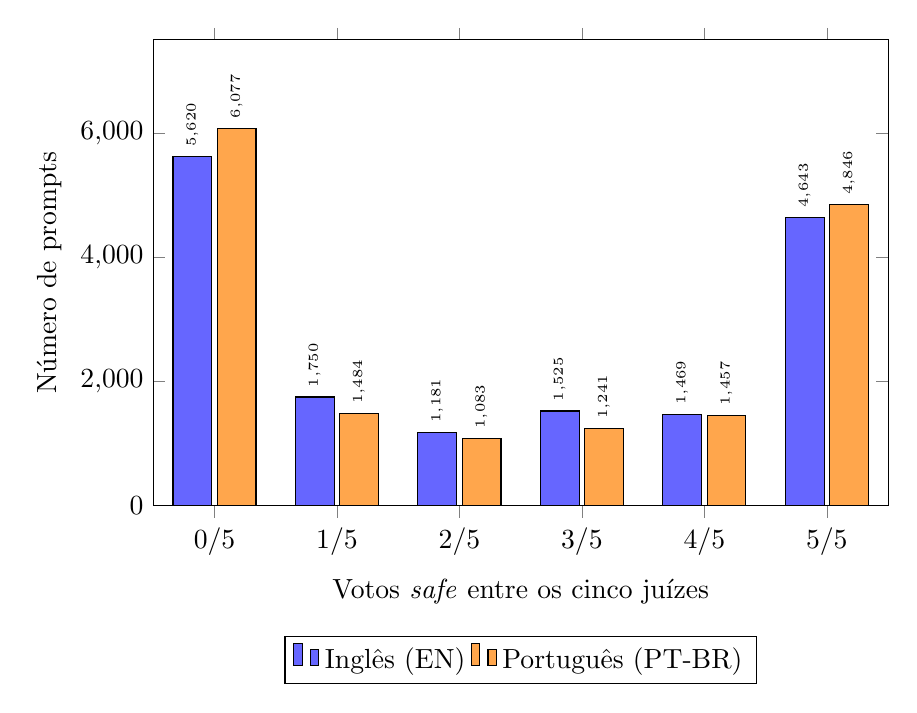
\begin{tikzpicture}
		\begin{axis}[
			ybar,
			bar width=14pt,
			width=0.9\textwidth,
			height=7.5cm,
			xlabel={Votos \textit{safe} entre os cinco juízes},
			ylabel={Número de prompts},
			xlabel style={yshift=-2pt},
			symbolic x coords={0/5, 1/5, 2/5, 3/5, 4/5, 5/5},
			xtick=data,
			ymin=0,
			ymax=7500,
			legend style={
				at={(0.5,-0.28)},
				anchor=north,
				legend columns=2
			},
			enlarge x limits=0.1,
			nodes near coords,
			every node near coord/.append style={
				font=\tiny,
				rotate=90,
				anchor=west,
			},
			]
			\addplot[fill=blue!60] coordinates {
				(0/5,5620) (1/5,1750) (2/5,1181) (3/5,1525) (4/5,1469) (5/5,4643)
			};
			\addplot[fill=orange!70] coordinates {
				(0/5,6077) (1/5,1484) (2/5,1083) (3/5,1241) (4/5,1457) (5/5,4846)
			};
			\legend{Inglês (EN), Português (PT-BR)}
		\end{axis}
	\end{tikzpicture}
	\caption{Distribuição dos votos \textit{safe} entre os cinco modelos juízes, em inglês e português}
	\label{fig:distribuicao-votos}
\end{figure}

\section{Modelos}
\label{sec:modelos}

Os cinco \textit{guardrails} avaliados neste trabalho foram selecionados com base em três critérios: disponibilidade pública no HuggingFace Hub com licença permissiva, compatibilidade com o modo de classificação de entrada via vLLM, e diversidade na estratégia de cobertura multilíngue. Essa diversidade é deliberada, pois permite investigar se o tipo de cobertura multilíngue do \textit{safety fine-tuning} influencia o \textit{gap} de desempenho em português brasileiro, conforme postulado na hipótese $H_1^2$.

Os modelos são classificados em duas categorias segundo sua estratégia de cobertura multilíngue no \textit{safety fine-tuning}. A primeira categoria, denominada \textbf{multilíngue nativa}, compreende modelos cujo \textit{safety fine-tuning} incluiu explicitamente o português brasileiro nos dados de treinamento: o \textbf{Llama Guard 3 8B} \cite{metallamaguard32024} e o \textbf{Llama Guard 3 1B} \cite{metallamaguard32024}, ambos desenvolvidos pela Meta sobre a arquitetura Llama 3, treinados nas categorias de risco do MLCommons em múltiplos idiomas incluindo PT-BR, e que operam retornando os rótulos \texttt{safe} ou \texttt{unsafe} seguidos das categorias violadas. A inclusão de ambos os tamanhos da família Llama Guard 3 permite investigar o efeito da escala de parâmetros sobre o \textit{gap} multilíngue sob quantização, conforme postulado na hipótese $H_1^3$.

A segunda categoria, denominada \textbf{base multilíngue com \textit{safety fine-tuning} sem PT-BR}, compreende modelos cujo modelo base possui capacidade multilíngue, mas cujo \textit{safety fine-tuning} não incluiu o português brasileiro de forma direta. Nessa categoria, o \textbf{ShieldGemma 9B} \cite{zeng2024shieldgemma}, desenvolvido pela Google sobre o Gemma 2, classifica prompts em quatro categorias de risco e retorna \texttt{Yes} ou \texttt{No} indicando violação das políticas de segurança fornecidas no prompt. O \textbf{Nemotron Safety Guard 8B} \cite{joshi2025cultureguard}, desenvolvido pela NVIDIA sobre o Llama 3.1 8B Instruct por meio de \textit{fine-tuning} com adaptadores LoRA, classifica prompts em 23 categorias de risco e retorna um JSON com o campo \texttt{User Safety}. O \textbf{Granite Guardian 4.1 8B} \cite{granite2024}, desenvolvido pela IBM sobre o Granite 4.1 8B, opera em modo de classificação binária por critério e retorna o veredicto em \texttt{<score>} \texttt{yes}/\texttt{no} \texttt{</score>}.

A Tabela~\ref{tab:modelos} sintetiza as principais características dos modelos avaliados.

\begin{table}[h!]
	\centering
	\Caption{\label{tab:modelos} Características dos \textit{guardrails} avaliados}
	\IBGEtab{}{
		\begin{tabular}{llll}
			\toprule
			\textbf{Modelo} & \textbf{Parâmetros} & \textbf{Cobertura multilíngue} & \textbf{Formato de saída} \\
			\midrule
			Llama Guard 3 8B  & 8B  & Multilíngue nativa & \texttt{safe}/\texttt{unsafe} + categorias \\
			Llama Guard 3 1B  & 1B  & Multilíngue nativa & \texttt{safe}/\texttt{unsafe} + categorias \\
			ShieldGemma 9B    & 9B  & Base multilíngue   & \texttt{Yes}/\texttt{No} \\
			Nemotron Safety 8B & 8B & Base multilíngue   & JSON (\texttt{User Safety}) \\
			Granite Guardian 4.1 8B & 8B & Base multilíngue & \texttt{<score>yes/no</score>} \\
			\bottomrule
		\end{tabular}
	}{
		\Fonte{Elaborado pelo autor.}
	}
\end{table}

\section{Quantização}
\label{sec:quantizacao}

A quantização é aplicada como fator de tratamento neste experimento, operacionalizando a variável independente principal. Adota-se o método GPTQ (\textit{Generalized Post-Training Quantization}) \cite{frantar2023gptq} em dois níveis de compressão: 8 \textit{bits} inteiros (INT8) e 4 \textit{bits} inteiros (INT4), complementados pelo \textit{baseline} em precisão original FP16. A escolha do GPTQ justifica-se por seu suporte nativo a múltiplos níveis de precisão no vLLM, garantindo consistência metodológica na comparação entre os níveis de quantização com um único método.

A quantização de 2 \textit{bits} foi deliberadamente excluída do experimento. Estudos anteriores demonstram que em precisões abaixo de 3 \textit{bits} a capacidade de raciocínio do modelo degrada de forma abrupta, tornando as predições essencialmente aleatórias e os resultados metodologicamente não informativos \cite{jaesik2025, kumar2024llmsnavigating}. O experimento concentra-se, portanto, nos níveis de quantização com relevância prática para implantação em produção.

Cada configuração de quantização é tratada como independente: os modelos são quantizados diretamente a partir dos pesos originais FP16, sem quantização progressiva entre níveis. Essa independência garante que os efeitos observados em cada nível sejam atribuíveis exclusivamente à compressão aplicada, sem acumulação de erros entre etapas.

O processo de quantização requer um conjunto de calibração para estimar a distribuição das ativações do modelo e minimizar o erro de reconstrução. Adota-se o corpus mC4 \cite{raffel2020exploring} como conjunto de calibração, composto por 256 amostras em inglês e 256 amostras em português brasileiro, selecionadas aleatoriamente, totalizando 512 amostras. A inclusão de amostras em português brasileiro no conjunto de calibração é motivada pela hipótese de que dados de calibração multilíngues preservam melhor as representações do modelo para idiomas não-ingleses, conforme sugerido por \citeonline{chimoto2026calibrating}. Os modelos quantizados são gerados com a biblioteca GPTQModel e disponibilizados publicamente no HuggingFace Hub para reprodutibilidade do experimento.

\section{Protocolo de Inferência}
\label{sec:protocolo}

O protocolo de inferência adotado neste trabalho segue o modo de classificação de entrada (\textit{input classification}), no qual cada \textit{guardrail} recebe exclusivamente o prompt do usuário como entrada e emite um julgamento binário de segurança, sem acesso a qualquer resposta gerada por um LLM subjacente. Esse modo é adotado quando o objetivo é interceptar conteúdo prejudicial antes do processamento pelo modelo principal, evitando que prompts maliciosos alcancem o LLM.

Para cada uma das 30 configurações experimentais, o script de inferência submete cada prompt do conjunto de dados ao \textit{guardrail} correspondente por meio de uma API compatível com o protocolo OpenAI, exposta pelo servidor vLLM \cite{kwon2023vllm}. O prompt não é enviado diretamente: ele é dinamicamente inserido no template nativo exigido por cada modelo antes da submissão, garantindo que a avaliação respeite o formato para o qual cada \textit{guardrail} foi treinado. Os templates específicos de cada modelo são descritos na Seção~\ref{sec:modelos}.

A extração da classificação binária é realizada por uma função de \textit{parsing} específica para cada modelo, dado que seus formatos de saída diferem entre si, conforme detalhado na Seção~\ref{sec:modelos}. Em todos os casos, respostas que não se enquadrem nos padrões esperados são registradas como \texttt{null} e contabilizadas separadamente ao final de cada configuração, sem atribuição de classe padrão, para evitar a introdução de viés nos resultados, conforme ilustrado na Figura~\ref{fig:pipeline-inferencia}.

\begin{figure}[h!]
	\Caption{\label{fig:pipeline-inferencia} Pipeline de inferência do experimento}
	\UFCfig{}{
		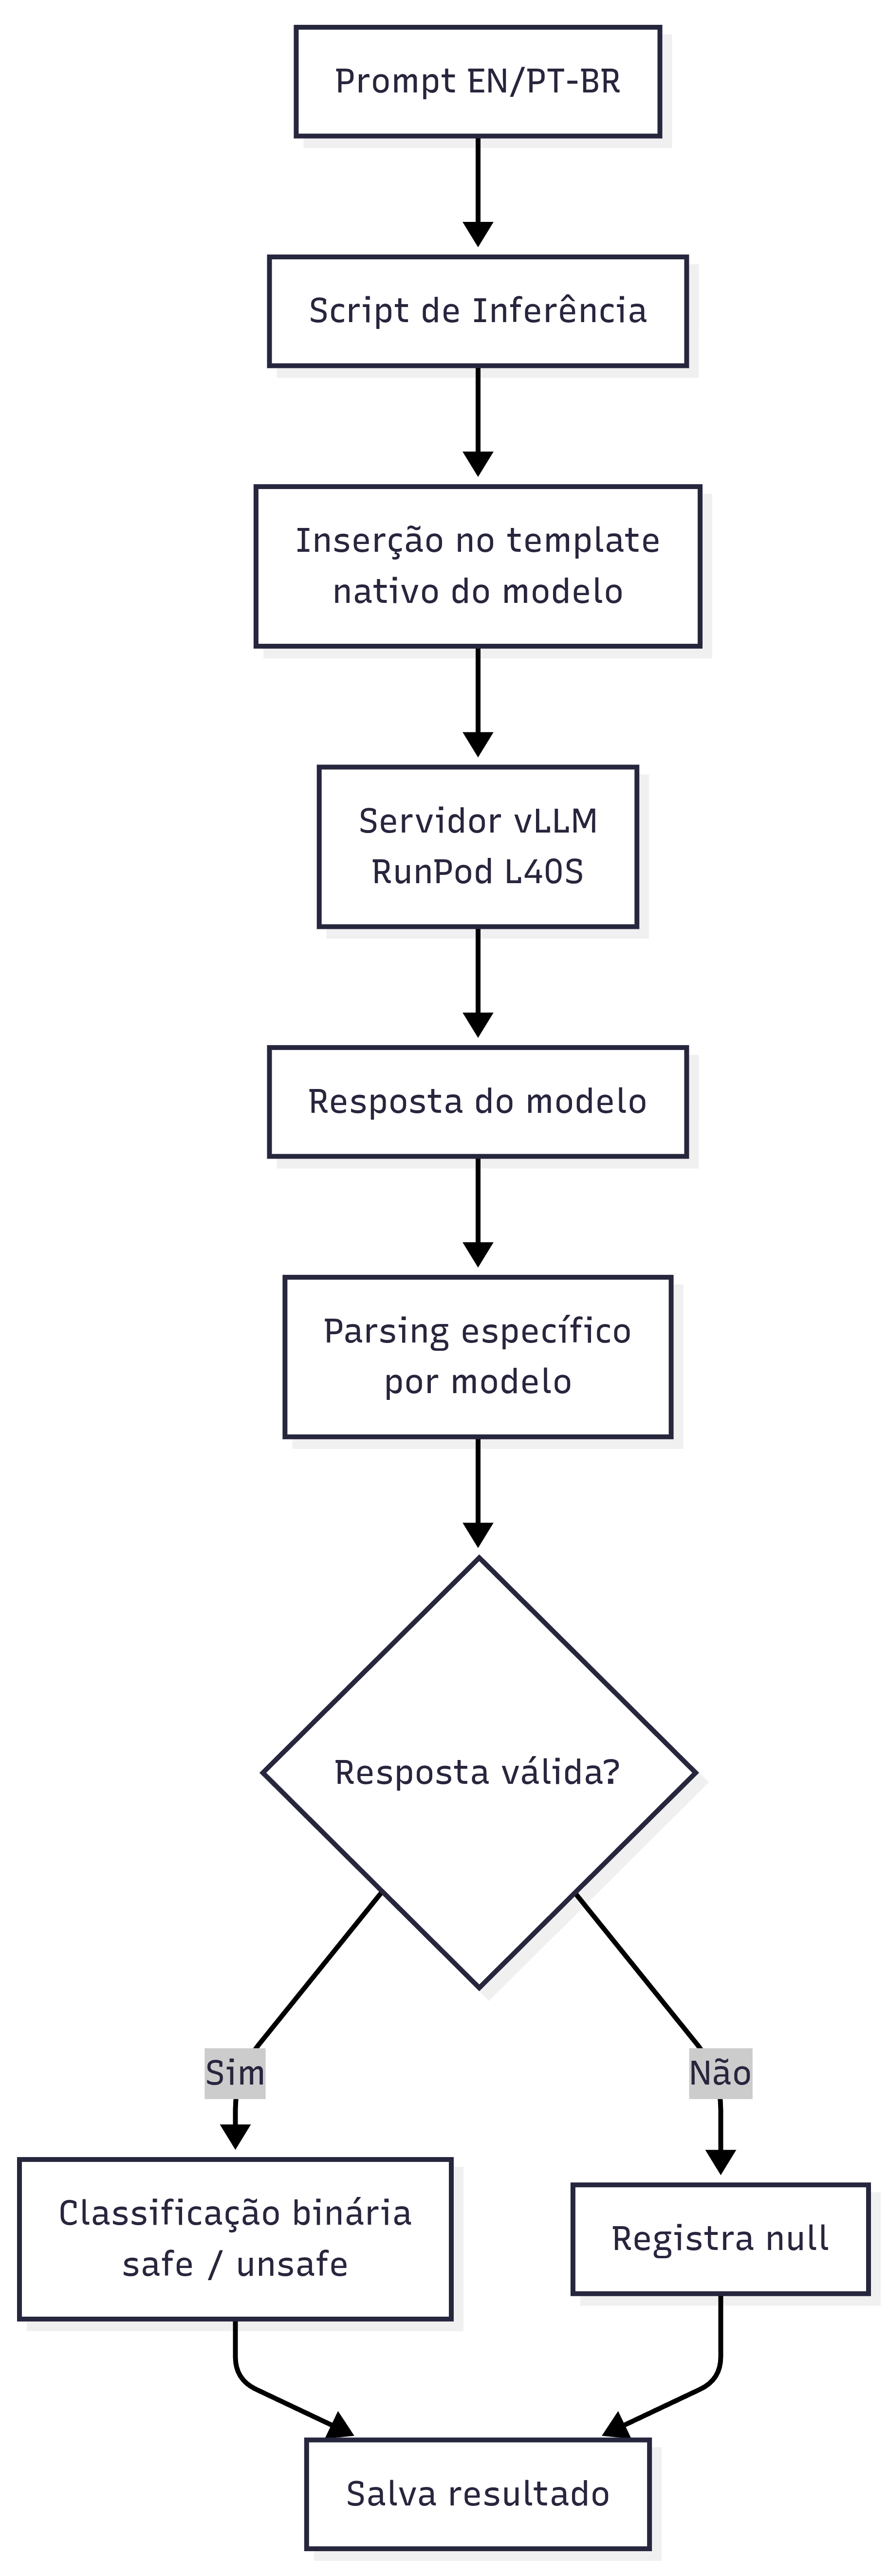
\includegraphics[width=0.4\textwidth]{figuras/pipeline-inferencia}
	}{
		\Fonte{Elaborado pelo autor.}
	}
\end{figure}

\subsection{Ambiente de Execução}
\label{sec:ambiente}

O experimento será executado em uma instância do RunPod Secure Cloud equipada com GPU NVIDIA L40S (arquitetura Ada Lovelace), 48 GB de VRAM, 94 GB de RAM e 16 vCPUs. O servidor de inferência utilizado é o vLLM, implantado por meio da imagem Docker oficial \texttt{vllm/vllm-openai:v0.9.0}, desenvolvida para GPUs NVIDIA com suporte a CUDA. Essa imagem inclui suporte nativo à quantização AWQ \cite{lin2024awq}, executada internamente pela biblioteca AutoAWQ, que permite a compressão dos pesos dos modelos para resoluções menores (como 8-bit e 4-bit), dispensando instalações adicionais e garantindo a reprodutibilidade do ambiente de execução. O servidor expõe uma API compatível com o protocolo OpenAI na porta 8000, permitindo que o script de inferência, executado localmente, submeta requisições ao modelo hospedado na instância remota sem alterações no código de coleta de dados.

Cada modelo é carregado individualmente na instância, servido e avaliado antes de ser substituído pela configuração seguinte. Esse procedimento garante isolamento completo entre as 30 configurações experimentais, eliminando interferências de estado entre modelos ou níveis de quantização distintos.

\subsection{Experimento Piloto}
\label{sec:piloto}
Antes da execução completa do experimento, será realizado um experimento piloto com um subconjunto de 100 prompts selecionados aleatoriamente do conjunto de dados, aplicado ao Llama Guard 3 8B em precisão base FP16, nos dois idiomas. O objetivo do piloto é validar o pipeline de ponta a ponta: verificar o correto carregamento do modelo no servidor vLLM, a formatação dos templates de prompt, o funcionamento do parsing das respostas e a estimativa do tempo total de execução do experimento completo. Eventuais falhas de formatação, erros de parsing ou comportamentos inesperados do modelo serão identificados e corrigidos nessa etapa, antes que o experimento seja executado nas 30 configurações completas. Os dados gerados no piloto são descartados e não integram os resultados do experimento.

\section{Métricas e Procedimentos de Análise}
\label{sec:metricas}

O desempenho de cada configuração experimental é mensurado por meio das métricas de precisão (\textit{precision}), revocação (\textit{recall}) e F1-\textit{score}, calculadas para a tarefa de classificação binária entre conteúdo seguro (\textit{safe}) e inseguro (\textit{unsafe}). A precisão mede a proporção de classificações positivas corretas sobre o total de classificações positivas realizadas, a revocação mede a proporção de positivos reais corretamente identificados, e o F1-\textit{score} é a média harmônica entre as duas, definido como:

\begin{equation}
	F1 = 2 \cdot \frac{\text{precision} \cdot \text{recall}}{\text{precision} + \text{recall}}
\end{equation}

Dado o desbalanceamento do conjunto de dados, com aproximadamente 88\% de instâncias inseguras e 12\% seguras, adota-se o F1 macro como métrica principal, calculado como a média não ponderada do F1 de cada classe. Essa escolha penaliza igualmente erros em ambas as classes independentemente de sua frequência, evitando que o desbalanceamento mascare falhas de desempenho na classe minoritária. A métrica derivada central deste trabalho é o $\Delta$F1, definido como:

\begin{equation}
	\Delta\text{F1} = \text{F1}_{\text{EN}} - \text{F1}_{\text{PT}}
\end{equation}

onde $\text{F1}_{\text{EN}}$ e $\text{F1}_{\text{PT}}$ correspondem ao F1 macro obtido pelo mesmo modelo na mesma configuração de quantização em inglês e em português brasileiro, respectivamente. Valores positivos de $\Delta$F1 indicam que o modelo performa melhor em inglês do que em português brasileiro.

Para quantificar a incerteza em torno de cada F1 sem necessidade de repetições do experimento, adota-se o método de \textit{bootstrap} com 1.000 iterações. Em cada iteração, reamostram-se com reposição os resultados de predição do modelo e calcula-se o F1 macro da amostra. O intervalo de confiança de 95\% é obtido pelos percentis 2,5\% e 97,5\% da distribuição empírica resultante \cite{efron1993bootstrap}. Todos os gráficos de resultado apresentam as estimativas de F1 acompanhadas de seus respectivos intervalos de confiança.

Para testar se o \textit{gap} de desempenho entre EN e PT-BR é estatisticamente significativo, aplica-se o teste de McNemar \cite{mcnemar1947} a cada par de configurações EN vs PT-BR. Para cada modelo e nível de quantização, monta-se uma tabela de contingência $2 \times 2$ com base nos acertos e erros em relação ao gabarito, contabilizando os casos em que o modelo acerta em EN mas erra em PT-BR ($n_{10}$) e os casos inversos ($n_{01}$). O teste avalia se a assimetria entre $n_{10}$ e $n_{01}$ é estatisticamente significativa, adotando $p < 0{,}05$ como nível de significância.

O gabarito utilizado em todas as métricas é a classificação gerada pelo modelo GPT-5 nano (\texttt{gpt-5-nano-2025-08-07}) aplicado diretamente aos prompts em inglês, conforme descrito na Seção~\ref{sec:dataset}. Essa escolha garante que o gabarito seja definido no nível do prompt, alinhado ao modo de classificação de entrada adotado neste experimento, e independente dos modelos avaliados. Como limitação, reconhece-se que o gabarito é produzido por outro LLM e não por anotação humana, o que é discutido nas ameaças à validade na Seção~\ref{sec:ameacas}.

\section{Ameaças à Validade}
\label{sec:ameacas}

Esta seção mapeia as principais ameaças à validade deste experimento, organizadas segundo as dimensões de validade interna, externa e de construto propostas por \citeonline{wohlin2012experimentation}.

\subsection{Validade Interna}
\label{sec:ameacas-interna}

A validade interna diz respeito à capacidade do experimento de medir corretamente os efeitos dos tratamentos sobre as variáveis dependentes, sem interferência de fatores externos não controlados.

A principal ameaça à validade interna é o uso do GPT-5 nano como classificador de gabarito, seguindo a abordagem \textit{LLM-as-a-Judge}. O gabarito não é produzido por anotação humana, o que significa que os rótulos de segurança refletem o julgamento de outro modelo de linguagem e podem conter vieses sistemáticos. Análises preliminares indicam que o GPT-5 nano tende a ser mais conservador do que a API de Moderação da OpenAI, classificando como \textit{unsafe} alguns prompts que seriam considerados \textit{safe} por outros sistemas. Esse conservadorismo pode introduzir falsos positivos no gabarito, afetando as métricas de precisão e F1 de todos os modelos avaliados de forma potencialmente uniforme, sem distorcer as comparações relativas entre modelos e idiomas.

A tradução automática dos prompts por meio da API do Google Translate representa uma segunda ameaça. Embora a tradução automática seja amplamente utilizada em estudos de segurança multilíngue \cite{yang2024benchmarking}, ela pode não preservar integralmente nuances semânticas, registros informais ou expressões culturais específicas do português brasileiro, podendo alterar o nível de risco percebido pelo \textit{guardrail}. Essa limitação é inerente à abordagem e está presente em trabalhos relacionados que adotam a mesma estratégia.

Por fim, identificaram-se duas anomalias pontuais na execução do experimento: 7 linhas corrompidas nos resultados do Nemotron Safety 8B, decorrentes de uma condição de corrida na escrita concorrente em disco, e 30 prompts com resposta vazia retornada pelo ShieldGemma 9B em inglês. Ambas as ocorrências foram tratadas como dados ausentes e excluídas da análise, representando menos de 0,2\% do total de instâncias e sem impacto significativo sobre as métricas.

\subsection{Validade Externa}
\label{sec:ameacas-externa}

A validade externa diz respeito à capacidade de generalização dos resultados para além do contexto experimental específico.

Os resultados deste trabalho são baseados exclusivamente no BeaverTails, um dataset de segurança coletado a partir de interações com modelos de linguagem em inglês. Embora o BeaverTails seja amplamente utilizado na literatura \cite{ji2023beavertails}, suas categorias de risco podem não cobrir formas de conteúdo prejudicial culturalmente específicas do contexto brasileiro, como discursos de ódio relacionados a grupos sociais, políticos ou regionais sem equivalente direto em inglês. Os resultados devem ser interpretados com cautela quanto à sua representatividade para cenários de moderação nativamente brasileiros.

A avaliação restringe-se ao português brasileiro como idioma não-inglês. Os padrões de degradação observados podem não generalizar para outros idiomas, especialmente os de menor recurso, cujo comportamento sob quantização pode ser distinto. Adicionalmente, os cinco modelos avaliados representam uma amostra do ecossistema de \textit{guardrails} disponíveis, e modelos não incluídos neste estudo podem apresentar comportamentos diferentes.

\subsection{Validade de Construto}
\label{sec:ameacas-construto}

A validade de construto diz respeito à adequação das métricas escolhidas para operacionalizar os conceitos investigados.

O F1 macro é adotado como métrica principal em razão do desbalanceamento do dataset (88,3\% \textit{unsafe}). Embora o F1 macro penalize igualmente erros em ambas as classes, ele pode mascarar diferenças de comportamento por classe — por exemplo, um modelo que acerta quase todos os prompts \textit{unsafe} mas erra sistematicamente os \textit{safe} pode apresentar F1 macro semelhante a um modelo mais equilibrado. A análise de precisão e revocação por classe, disponível no material suplementar, oferece uma perspectiva complementar.

O $\Delta$F1 pressupõe que o F1 é comparável entre idiomas no mesmo gabarito, isto é, que os prompts em inglês e em português brasileiro têm dificuldade equivalente para os modelos. Essa premissa pode ser violada se a tradução introduzir sistematicamente prompts mais ou menos ambíguos em PT-BR, distorcendo a comparação. A análise por categorias de conteúdo, discutida nos resultados, permite identificar se eventuais distorções se concentram em categorias específicas.

\section{Cronograma}
\label{sec:cronograma}

O cronograma de execução das atividades previstas para o TCC 2 é apresentado na Tabela~\ref{tab:cronograma}. O planejamento concentra o desenvolvimento prático nos primeiros meses, reservando a etapa final exclusivamente para análise e documentação.

\begin{table}[h!]
	\Caption{\label{tab:cronograma} Cronograma de execução do TCC 2}
	\IBGEtab{}{
		\begin{tabular}{lcccccc}
			\toprule
			\textbf{Atividade} & \textbf{Ago} & \textbf{Set} & \textbf{Out} & \textbf{Nov} & \textbf{Dez} \\
			\midrule
			Revisão bibliográfica e ajustes teóricos & X & X & & & \\
			Quantização dos modelos (GPTQ 8bit e 4bit) & X & X & & & \\
			Execução do experimento completo & & X & X & & \\
			Análise e discussão dos resultados & & & X & X & \\
			Redação e revisão final do TCC 2 & & & & X & X \\
			Defesa do TCC 2 & & & & & X \\
			\bottomrule
		\end{tabular}
	}{
		\Fonte{Elaborado pelo autor.}
	}
\end{table}